\chapter{Point-of-Care Ultrasound (POCUS)}
\label{ch:pocus}

% Chapter-opening illustrated modality infographic.
\begin{center}
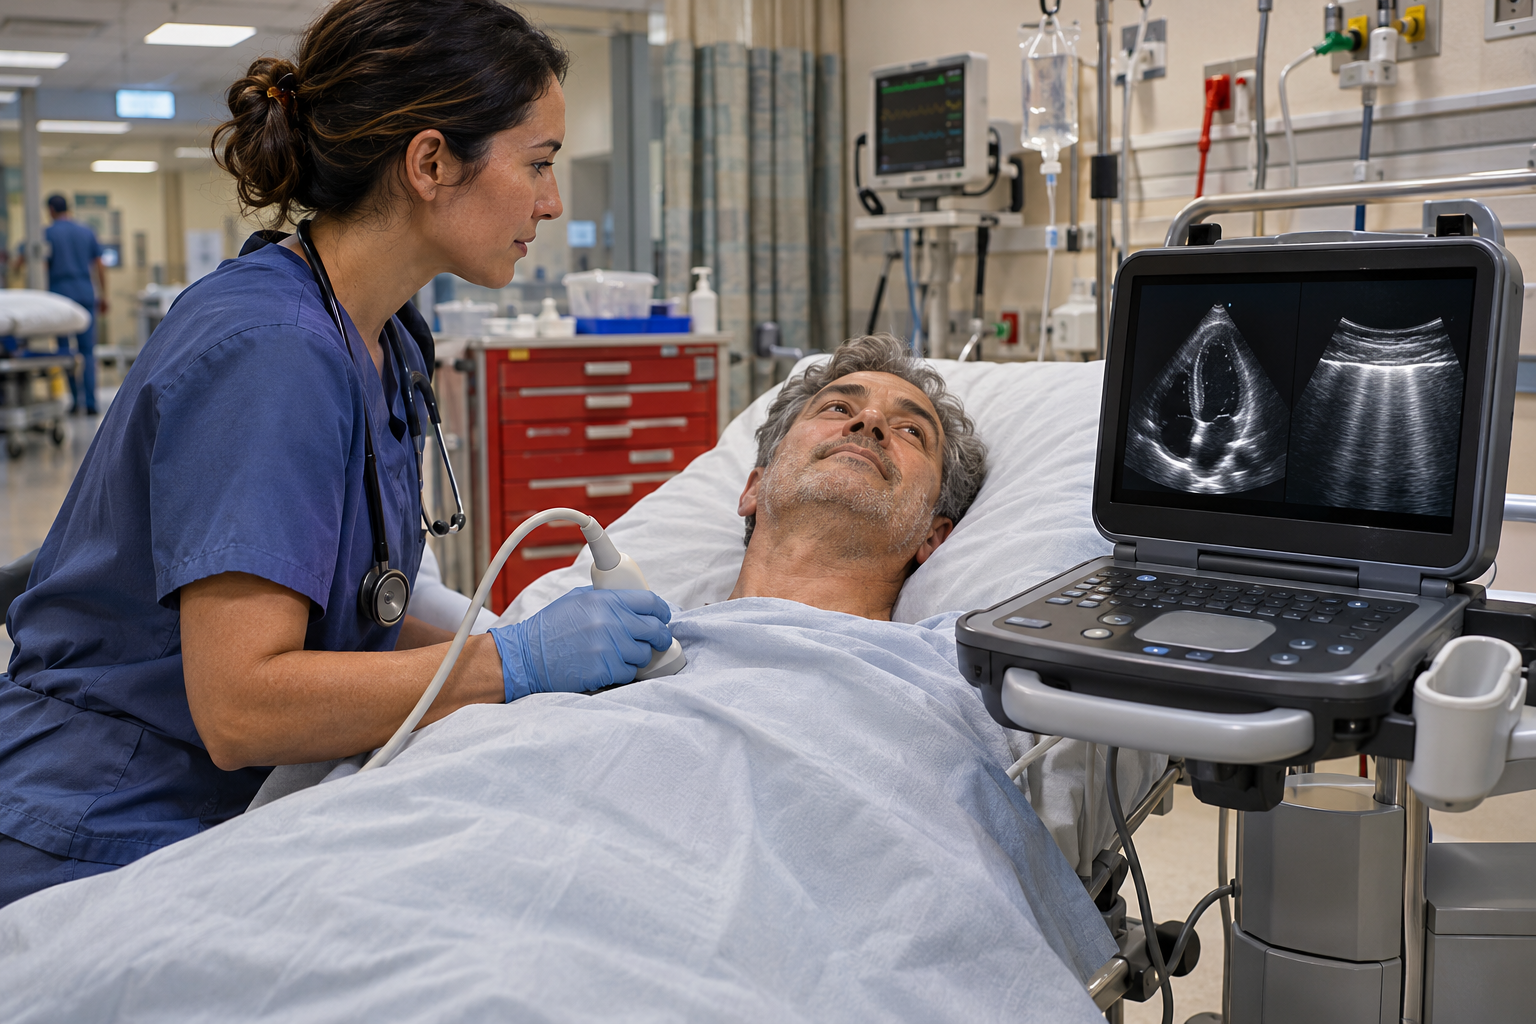
\includegraphics[width=\textwidth,keepaspectratio]{modalities/infographics/pocus_realistic.png}
\end{center}
\begin{center}\footnotesize POCUS is a focused bedside scan used to answer a defined clinical question; it does not replace a comprehensive examination when one is needed. AI-generated illustration; ultrasound panels are not clinical studies.\end{center}

\section{Overview}
Point-of-care ultrasound (POCUS) is a focused ultrasound examination performed and interpreted by a healthcare professional at the patient's bedside to answer specific clinical questions, guide procedures or monitor physiological changes.

Unlike comprehensive diagnostic ultrasonography, POCUS generally investigates a limited set of abnormalities to support immediate clinical decision-making. It is widely used in emergency medicine, critical care, anesthesiology, internal medicine, trauma care and rural healthcare.

\section{Where point-of-care ultrasound is used}

\subsection{Cardiovascular diseases}
\begin{enumerate}[leftmargin=*,itemsep=0.45em,topsep=0.4em]
\item \textbf{Acute myocardial infarction.} Useful imaging findings include: Possible regional wall motion abnormalities; requires clinical and diagnostic testing for assessment.
\item \textbf{Cardiac arrest.} Useful imaging findings include: Absence or presence of myocardial motion.
\item \textbf{Cardiac tamponade.} Useful imaging findings include: Pericardial effusion with right atrial or right ventricular collapse.
\item \textbf{Cardiogenic shock.} Useful imaging findings include: Reduced ventricular contractility or other cardiac abnormalities.
\item \textbf{Congestive heart failure.} Useful imaging findings include: Ventricular dysfunction, possible pulmonary B-lines and venous congestion.
\item \textbf{Dilated cardiomyopathy.} Useful imaging findings include: Enlarged ventricular chambers with reduced contractility.
\item \textbf{Hypertrophic cardiomyopathy.} Useful imaging findings include: Abnormal myocardial thickening.
\item \textbf{Hypovolemic shock.} Useful imaging findings include: Small, hyperdynamic left ventricle in selected patients.
\item \textbf{Infective endocarditis.} Useful imaging findings include: Possible visible vegetation; absence on POCUS does not exclude endocarditis, and comprehensive echocardiography is required.
\item \textbf{Intracardiac thrombus.} Useful imaging findings include: Possible abnormal intracardiac echogenic mass requiring confirmation with comprehensive imaging.
\item \textbf{Left ventricular aneurysm.} Useful imaging findings include: Focal ventricular wall thinning and abnormal motion.
\item \textbf{Left ventricular systolic dysfunction.} Useful imaging findings include: Reduced myocardial contractility.
\item \textbf{Obstructive shock.} Useful imaging findings include: Findings suggesting tamponade, pulmonary embolism or another obstruction.
\item \textbf{Pericardial effusion.} Useful imaging findings include: Anechoic fluid surrounding the heart.
\item \textbf{Pulmonary embolism.} Useful imaging findings include: Possible right ventricular dilatation and septal flattening; these indirect findings do not diagnose or exclude pulmonary embolism.
\item \textbf{Right ventricular dilatation.} Useful imaging findings include: Increased right-to-left ventricular size ratio.
\item \textbf{Right ventricular dysfunction.} Useful imaging findings include: Reduced right ventricular contractility.
\item \textbf{Septic shock.} Useful imaging findings include: Hyperdynamic or depressed ventricular contractility.
\item \textbf{Severe aortic stenosis.} Useful imaging findings include: Restricted or calcified aortic valve leaflets may raise suspicion; severity requires comprehensive echocardiography.
\item \textbf{Severe mitral regurgitation.} Useful imaging findings include: Possible abnormal regurgitant flow on color Doppler; severity requires comprehensive echocardiography.
\end{enumerate}
Focused cardiac ultrasound may raise suspicion for regional wall-motion abnormalities, vegetations, intracardiac thrombus or valve disease, but does not establish these diagnoses or reliably grade valve severity. Comprehensive echocardiography and clinical assessment are needed when these findings are suspected. A negative focused examination cannot exclude myocardial infarction, pulmonary embolism, endocarditis or significant valvular disease.

\subsection{Pulmonary and pleural diseases}
\begin{enumerate}[leftmargin=*,itemsep=0.45em,topsep=0.4em]
\item \textbf{Acute respiratory distress syndrome (ARDS).} Useful imaging findings include: Heterogeneous B-lines, irregular pleural line and spared regions.
\item \textbf{Aspiration pneumonia.} Useful imaging findings include: Dependent pulmonary consolidation.
\item \textbf{Cardiogenic pulmonary edema.} Useful imaging findings include: Frequently diffuse bilateral B-lines with relatively smooth pleural line.
\item \textbf{Diaphragmatic dysfunction.} Useful imaging findings include: Reduced diaphragmatic excursion or thickening.
\item \textbf{Diaphragmatic paralysis.} Useful imaging findings include: Absent or paradoxical diaphragmatic movement.
\item \textbf{Empyema.} Useful imaging findings include: Complex pleural collection with septations.
\item \textbf{Hemothorax.} Useful imaging findings include: Pleural fluid with variable internal echoes.
\item \textbf{Interstitial lung disease.} Useful imaging findings include: Multiple B-lines and pleural irregularities.
\item \textbf{Peripheral pulmonary abscess.} Useful imaging findings include: Complex fluid-containing pulmonary lesion accessible to ultrasound.
\item \textbf{Pleural effusion.} Useful imaging findings include: Anechoic or complex fluid above the diaphragm.
\item \textbf{Pleural malignancy.} Useful imaging findings include: Possible pleural nodularity and effusion.
\item \textbf{Pleural thickening.} Useful imaging findings include: Abnormally thickened pleural line.
\item \textbf{Pneumonia.} Useful imaging findings include: Subpleural consolidation with possible dynamic air bronchograms.
\item \textbf{Pneumothorax.} Useful imaging findings include: Absent lung sliding, absent B-lines and possible lung point.
\item \textbf{Pulmonary atelectasis.} Useful imaging findings include: Tissue-like consolidation with possible static air bronchograms.
\item \textbf{Pulmonary contusion.} Useful imaging findings include: Focal B-lines and subpleural consolidation.
\item \textbf{Pulmonary edema.} Useful imaging findings include: Multiple bilateral B-lines.
\item \textbf{Pulmonary fibrosis.} Useful imaging findings include: Irregular pleural surface and B-lines.
\item \textbf{Pulmonary infarction.} Useful imaging findings include: Possible peripheral wedge-shaped subpleural lesion.
\item \textbf{Viral pneumonia.} Useful imaging findings include: Patchy B-lines and subpleural abnormalities.
\end{enumerate}
Lung ultrasound primarily evaluates the pleural interface, artifacts and abnormalities extending to the lung periphery. It cannot comprehensively visualize normally aerated lung parenchyma.

\subsection{Vascular diseases}
\begin{enumerate}[leftmargin=*,itemsep=0.45em,topsep=0.4em]
\item \textbf{Abdominal aortic aneurysm.} Useful imaging findings include: Abdominal aortic diameter of at least 3 cm.
\item \textbf{Acute limb ischemia.} Useful imaging findings include: Reduced or absent arterial Doppler signals.
\item \textbf{Aortic dissection.} Useful imaging findings include: Possible intimal flap separating vascular lumens.
\item \textbf{Arterial pseudoaneurysm.} Useful imaging findings include: Vascular sac with characteristic to-and-fro flow at its neck.
\item \textbf{Arterial thrombosis.} Useful imaging findings include: Intraluminal material with absent or reduced flow.
\item \textbf{Arteriovenous fistula.} Useful imaging findings include: Abnormal communication with turbulent blood flow.
\item \textbf{Central venous congestion.} Useful imaging findings include: Venous dilatation and abnormal Doppler waveforms.
\item \textbf{Deep vein thrombosis.} Useful imaging findings include: Failure of venous compression.
\item \textbf{Femoral vein thrombosis.} Useful imaging findings include: Noncompressible femoral vein.
\item \textbf{Hepatic venous congestion.} Useful imaging findings include: Abnormal hepatic venous Doppler waveform.
\item \textbf{Iliac artery aneurysm.} Useful imaging findings include: Abnormal arterial dilatation.
\item \textbf{Peripheral arterial disease.} Useful imaging findings include: Abnormal arterial waveforms and vascular calcification.
\item \textbf{Popliteal vein thrombosis.} Useful imaging findings include: Noncompressible popliteal vein.
\item \textbf{Portal venous congestion.} Useful imaging findings include: Increased portal vein pulsatility.
\item \textbf{Renal venous congestion.} Useful imaging findings include: Discontinuous intrarenal venous flow.
\item \textbf{Superficial thrombophlebitis.} Useful imaging findings include: Noncompressible superficial vein with surrounding inflammation.
\item \textbf{Upper-extremity venous thrombosis.} Useful imaging findings include: Noncompressibility or abnormal venous Doppler flow.
\end{enumerate}
A negative focused ultrasound examination cannot reliably exclude aortic dissection or all forms of deep vein thrombosis.

\subsection{Trauma-related conditions}
\begin{enumerate}[leftmargin=*,itemsep=0.45em,topsep=0.4em]
\item \textbf{Abdominal wall hematoma.} Useful imaging findings include: Localized heterogeneous fluid collection.
\item \textbf{Hemoperitoneum.} Useful imaging findings include: Free intraperitoneal fluid.
\item \textbf{Hepatic injury.} Useful imaging findings include: Possible perihepatic fluid or abnormal hepatic echotexture.
\item \textbf{Intra-abdominal hemorrhage.} Useful imaging findings include: Free fluid in dependent abdominal spaces.
\item \textbf{Long-bone fracture.} Useful imaging findings include: Disruption of the hyperechoic bone surface.
\item \textbf{Renal trauma.} Useful imaging findings include: Possible perinephric fluid or hematoma.
\item \textbf{Rib fracture.} Useful imaging findings include: Discontinuity of the rib cortex.
\item \textbf{Splenic injury.} Useful imaging findings include: Possible perisplenic fluid or heterogeneous splenic tissue.
\item \textbf{Sternal fracture.} Useful imaging findings include: Cortical interruption or displacement.
\item \textbf{Traumatic cardiac tamponade.} Useful imaging findings include: Pericardial fluid with signs of impaired cardiac filling.
\item \textbf{Traumatic hemopericardium.} Useful imaging findings include: Pericardial fluid following trauma.
\item \textbf{Traumatic hemothorax.} Useful imaging findings include: Fluid within the pleural cavity.
\item \textbf{Traumatic muscle injury.} Useful imaging findings include: Disrupted muscle fibers and hematoma.
\item \textbf{Traumatic pneumothorax.} Useful imaging findings include: Abnormal lung sliding with possible lung point.
\end{enumerate}
FAST and eFAST primarily identify free fluid and selected thoracic abnormalities rather than directly identifying every injured organ. A negative examination does not exclude significant trauma.

\subsection{Hepatic and hepatobiliary diseases}
\begin{enumerate}[leftmargin=*,itemsep=0.45em,topsep=0.4em]
\item \textbf{Acalculous cholecystitis.} Useful imaging findings include: Gallbladder distension and inflammatory changes without stones.
\item \textbf{Acute cholecystitis.} Useful imaging findings include: Gallstones, wall thickening, pericholecystic fluid and sonographic Murphy sign.
\item \textbf{Ascites.} Useful imaging findings include: Free intraperitoneal fluid.
\item \textbf{Biliary obstruction.} Useful imaging findings include: Dilatation of the biliary tract.
\item \textbf{Choledocholithiasis.} Useful imaging findings include: Possible echogenic stone within the common bile duct.
\item \textbf{Cholelithiasis.} Useful imaging findings include: Echogenic gallstones with posterior acoustic shadowing.
\item \textbf{Gallbladder hydrops.} Useful imaging findings include: Marked gallbladder distension.
\item \textbf{Gallbladder sludge.} Useful imaging findings include: Low-level dependent intraluminal echoes.
\item \textbf{Hepatic abscess.} Useful imaging findings include: Complex heterogeneous fluid collection.
\item \textbf{Hepatic cyst.} Useful imaging findings include: Anechoic lesion with posterior acoustic enhancement.
\item \textbf{Hepatic steatosis.} Useful imaging findings include: Increased hepatic echogenicity.
\item \textbf{Hepatomegaly.} Useful imaging findings include: Increased liver dimensions.
\item \textbf{Liver cirrhosis.} Useful imaging findings include: Nodular hepatic surface and coarse echotexture.
\item \textbf{Portal hypertension.} Useful imaging findings include: Possible collateral vessels, splenomegaly and ascites.
\end{enumerate}

\subsection{Renal and urinary tract diseases}
\begin{enumerate}[leftmargin=*,itemsep=0.45em,topsep=0.4em]
\item \textbf{Acute kidney injury.} Useful imaging findings include: Possible obstruction or other structural renal abnormalities.
\item \textbf{Benign prostatic hyperplasia.} Useful imaging findings include: Enlarged prostate and possible urinary retention.
\item \textbf{Bladder blood clot.} Useful imaging findings include: Intraluminal echogenic material without internal vascularity.
\item \textbf{Bladder calculus.} Useful imaging findings include: Mobile echogenic structure with acoustic shadowing.
\item \textbf{Bladder diverticulum.} Useful imaging findings include: Fluid-filled outpouching communicating with the bladder.
\item \textbf{Bladder outlet obstruction.} Useful imaging findings include: Increased residual urine volume.
\item \textbf{Chronic kidney disease.} Useful imaging findings include: Small kidneys, increased echogenicity or cortical thinning.
\item \textbf{Hydronephrosis.} Useful imaging findings include: Dilatation of the renal collecting system.
\item \textbf{Nephrolithiasis.} Useful imaging findings include: Echogenic renal stone with acoustic shadowing.
\item \textbf{Obstructive uropathy.} Useful imaging findings include: Collecting system dilatation or bladder distension.
\item \textbf{Perinephric abscess.} Useful imaging findings include: Abnormal fluid collection surrounding the kidney.
\item \textbf{Polycystic kidney disease.} Useful imaging findings include: Multiple bilateral renal cysts.
\item \textbf{Renal abscess.} Useful imaging findings include: Focal complex fluid collection.
\item \textbf{Simple renal cyst.} Useful imaging findings include: Well-defined anechoic lesion.
\item \textbf{Ureterolithiasis.} Useful imaging findings include: Possible visible ureteral calculus and upstream hydronephrosis.
\item \textbf{Urinary retention.} Useful imaging findings include: Distended urinary bladder.
\end{enumerate}
POCUS is useful for detecting urinary obstruction but generally cannot establish the cause of intrinsic kidney disease.

\subsection{Gastrointestinal diseases}
\begin{enumerate}[leftmargin=*,itemsep=0.45em,topsep=0.4em]
\item \textbf{Acute appendicitis.} Useful imaging findings include: Enlarged, noncompressible blind-ending tubular structure.
\item \textbf{Acute diverticulitis.} Useful imaging findings include: Focal bowel wall thickening and inflamed surrounding fat.
\item \textbf{Appendiceal abscess.} Useful imaging findings include: Complex periappendiceal fluid collection.
\item \textbf{Appendicolith.} Useful imaging findings include: Echogenic appendiceal focus with posterior shadowing.
\item \textbf{Bowel ischemia.} Useful imaging findings include: Abnormal wall thickness, peristalsis or perfusion.
\item \textbf{Crohn disease.} Useful imaging findings include: Segmental bowel wall thickening and possible hypervascularity.
\item \textbf{Gastroenteritis.} Useful imaging findings include: Nonspecific fluid-filled loops and altered peristalsis.
\item \textbf{Gastrointestinal perforation.} Useful imaging findings include: Possible abnormal free-air artifacts.
\item \textbf{Hypertrophic pyloric stenosis.} Useful imaging findings include: Thickened and elongated pyloric muscle.
\item \textbf{Incarcerated hernia.} Useful imaging findings include: Nonreducible herniated contents.
\item \textbf{Inguinal hernia.} Useful imaging findings include: Protrusion of abdominal contents through an inguinal defect.
\item \textbf{Intra-abdominal abscess.} Useful imaging findings include: Localized complex fluid collection.
\item \textbf{Intussusception.} Useful imaging findings include: Target or doughnut sign.
\item \textbf{Large bowel obstruction.} Useful imaging findings include: Colonic dilatation.
\item \textbf{Paralytic ileus.} Useful imaging findings include: Dilated bowel loops with reduced peristalsis.
\item \textbf{Small bowel obstruction.} Useful imaging findings include: Dilated fluid-filled bowel loops with abnormal peristalsis.
\item \textbf{Ulcerative colitis.} Useful imaging findings include: Colonic wall thickening.
\item \textbf{Umbilical hernia.} Useful imaging findings include: Abdominal contents extending through an umbilical defect.
\end{enumerate}

\subsection{Obstetric diseases and conditions}
\begin{enumerate}[leftmargin=*,itemsep=0.45em,topsep=0.4em]
\item \textbf{Anembryonic pregnancy.} Useful imaging findings include: Empty gestational sac meeting diagnostic size criteria.
\item \textbf{Breech presentation.} Useful imaging findings include: Fetal buttocks or feet directed toward the cervix.
\item \textbf{Early pregnancy loss.} Useful imaging findings include: Findings meeting validated criteria for pregnancy nonviability.
\item \textbf{Ectopic pregnancy.} Useful imaging findings include: Possible extrauterine gestational sac or adnexal mass.
\item \textbf{Fetal cardiac activity.} Useful imaging findings include: Visible rhythmic fetal cardiac motion.
\item \textbf{Intrauterine fetal demise.} Useful imaging findings include: Absent fetal cardiac activity meeting confirmation requirements.
\item \textbf{Intrauterine pregnancy.} Useful imaging findings include: Intrauterine gestational sac containing a yolk sac or embryo.
\item \textbf{Low-lying placenta.} Useful imaging findings include: Possible placental edge near the internal cervical opening; confirm with dedicated obstetric ultrasound.
\item \textbf{Molar pregnancy.} Useful imaging findings include: Abnormal heterogeneous intrauterine tissue with cystic spaces.
\item \textbf{Multiple pregnancy.} Useful imaging findings include: Multiple embryos or gestational sacs.
\item \textbf{Oligohydramnios.} Useful imaging findings include: Reduced amniotic fluid volume.
\item \textbf{Placenta previa.} Useful imaging findings include: Possible placenta covering the internal cervical opening on a bedside scan; confirm with dedicated obstetric ultrasound.
\item \textbf{Polyhydramnios.} Useful imaging findings include: Increased amniotic fluid volume.
\item \textbf{Pregnancy of unknown location.} Useful imaging findings include: No definite intrauterine or extrauterine pregnancy identified.
\item \textbf{Retained products of conception.} Useful imaging findings include: Abnormal intrauterine tissue with variable vascularity.
\item \textbf{Ruptured ectopic pregnancy.} Useful imaging findings include: Possible adnexal abnormality with hemoperitoneum.
\item \textbf{Subchorionic hematoma.} Useful imaging findings include: Crescent-shaped collection adjacent to the gestational sac.
\item \textbf{Transverse fetal lie.} Useful imaging findings include: Fetal longitudinal axis perpendicular to maternal axis.
\end{enumerate}
POCUS does not replace comprehensive antenatal ultrasound, fetal anomaly screening or formal assessment of uncertain pregnancy viability. Suspected placenta previa or low-lying placenta requires dedicated obstetric imaging; transvaginal ultrasound may be needed for accurate localization.

\subsection{Gynecological diseases}
\begin{enumerate}[leftmargin=*,itemsep=0.45em,topsep=0.4em]
\item \textbf{Adenomyosis.} Useful imaging findings include: Heterogeneous myometrium with possible small cystic spaces.
\item \textbf{Endometrial thickening.} Useful imaging findings include: Increased endometrial thickness.
\item \textbf{Hematometra.} Useful imaging findings include: Fluid or blood distending the endometrial cavity.
\item \textbf{Hemorrhagic ovarian cyst.} Useful imaging findings include: Reticular internal echoes or retracting clot.
\item \textbf{Hydrosalpinx.} Useful imaging findings include: Elongated fluid-filled tubular adnexal structure.
\item \textbf{Ovarian endometrioma.} Useful imaging findings include: Homogeneous low-level internal echoes.
\item \textbf{Ovarian torsion.} Useful imaging findings include: Enlarged ovary with peripheral follicles and possible twisted vascular pedicle.
\item \textbf{Pelvic inflammatory disease.} Useful imaging findings include: Possible tubal thickening and pelvic fluid.
\item \textbf{Ruptured ovarian cyst.} Useful imaging findings include: Adnexal lesion with pelvic free fluid.
\item \textbf{Simple ovarian cyst.} Useful imaging findings include: Anechoic adnexal lesion.
\item \textbf{Tubo-ovarian abscess.} Useful imaging findings include: Complex inflammatory adnexal mass.
\item \textbf{Uterine fibroids.} Useful imaging findings include: Well-defined solid myometrial masses.
\end{enumerate}
Preserved ovarian Doppler flow does not exclude ovarian torsion.

\subsection{Male reproductive disorders}
\begin{enumerate}[leftmargin=*,itemsep=0.45em,topsep=0.4em]
\item \textbf{Epididymal cyst.} Useful imaging findings include: Well-defined anechoic epididymal lesion.
\item \textbf{Epididymitis.} Useful imaging findings include: Enlarged hypervascular epididymis.
\item \textbf{Epididymo-orchitis.} Useful imaging findings include: Increased epididymal and testicular vascularity.
\item \textbf{Hematocele.} Useful imaging findings include: Complex hemorrhagic scrotal fluid collection.
\item \textbf{Hydrocele.} Useful imaging findings include: Anechoic fluid surrounding the testis.
\item \textbf{Orchitis.} Useful imaging findings include: Enlarged hypervascular testis.
\item \textbf{Pyocele.} Useful imaging findings include: Complex infected scrotal collection.
\item \textbf{Testicular hematoma.} Useful imaging findings include: Focal heterogeneous intratesticular collection.
\item \textbf{Testicular mass.} Useful imaging findings include: Discrete intratesticular lesion.
\item \textbf{Testicular rupture.} Useful imaging findings include: Disrupted testicular contour and heterogeneous parenchyma.
\item \textbf{Testicular torsion.} Useful imaging findings include: Reduced or absent testicular perfusion and possible whirlpool sign.
\item \textbf{Varicocele.} Useful imaging findings include: Dilated pampiniform venous plexus.
\end{enumerate}

\subsection{Musculoskeletal diseases}
\begin{enumerate}[leftmargin=*,itemsep=0.45em,topsep=0.4em]
\item \textbf{Achilles tendinopathy.} Useful imaging findings include: Tendon thickening and altered fibrillar architecture.
\item \textbf{Achilles tendon rupture.} Useful imaging findings include: Tendon discontinuity and retraction.
\item \textbf{Baker cyst.} Useful imaging findings include: Fluid collection between characteristic posterior knee structures.
\item \textbf{Bursitis.} Useful imaging findings include: Fluid within a bursal space.
\item \textbf{Calcific tendinitis.} Useful imaging findings include: Echogenic intratendinous calcification.
\item \textbf{Calcium pyrophosphate deposition disease.} Useful imaging findings include: Hyperechoic deposits within cartilage.
\item \textbf{Clavicle fracture.} Useful imaging findings include: Cortical discontinuity.
\item \textbf{Foreign body.} Useful imaging findings include: Echogenic structure with variable shadowing or reverberation.
\item \textbf{Gout.} Useful imaging findings include: Double-contour sign and possible tophaceous deposits.
\item \textbf{Joint effusion.} Useful imaging findings include: Anechoic or hypoechoic intra-articular fluid.
\item \textbf{Muscle hematoma.} Useful imaging findings include: Heterogeneous intramuscular collection.
\item \textbf{Muscle tear.} Useful imaging findings include: Disruption of normal muscle fibers.
\item \textbf{Osteoarthritis.} Useful imaging findings include: Osteophytes and irregular articular margins.
\item \textbf{Patellar tendon rupture.} Useful imaging findings include: Discontinuity of patellar tendon fibers.
\item \textbf{Plantar fasciitis.} Useful imaging findings include: Thickened hypoechoic plantar fascia.
\item \textbf{Quadriceps tendon rupture.} Useful imaging findings include: Disrupted quadriceps tendon architecture.
\item \textbf{Radial head fracture.} Useful imaging findings include: Cortical disruption or associated joint effusion.
\item \textbf{Rheumatoid arthritis.} Useful imaging findings include: Synovial hypertrophy and increased Doppler vascularity.
\item \textbf{Rotator cuff tear.} Useful imaging findings include: Focal tendon defect or complete discontinuity.
\item \textbf{Rotator cuff tendinopathy.} Useful imaging findings include: Tendon thickening and heterogeneous echogenicity.
\item \textbf{Septic arthritis.} Useful imaging findings include: Joint effusion with possible synovial inflammatory changes.
\item \textbf{Shoulder dislocation.} Useful imaging findings include: Abnormal humeral head position relative to glenoid.
\item \textbf{Tenosynovitis.} Useful imaging findings include: Tendon sheath fluid and increased vascularity.
\item \textbf{Trigger finger.} Useful imaging findings include: A1 pulley thickening and abnormal tendon movement.
\end{enumerate}
Ultrasound cannot reliably distinguish septic arthritis from sterile inflammatory joint effusions without clinical assessment and, when indicated, joint aspiration.

\subsection{Skin and soft-tissue diseases}
\begin{enumerate}[leftmargin=*,itemsep=0.45em,topsep=0.4em]
\item \textbf{Cellulitis.} Useful imaging findings include: Cobblestone appearance of subcutaneous tissue.
\item \textbf{Cutaneous abscess.} Useful imaging findings include: Complex fluid collection with internal debris.
\item \textbf{Epidermoid cyst.} Useful imaging findings include: Well-defined lesion with variable internal echoes.
\item \textbf{Hidradenitis suppurativa.} Useful imaging findings include: Dermal thickening, fluid collections and sinus tracts.
\item \textbf{Lipoma.} Useful imaging findings include: Relatively well-defined superficial fatty lesion.
\item \textbf{Necrotizing fasciitis.} Useful imaging findings include: Possible fascial fluid, thickening or soft-tissue gas.
\item \textbf{Pilonidal abscess.} Useful imaging findings include: Complex subcutaneous collection near the natal cleft.
\item \textbf{Pyomyositis.} Useful imaging findings include: Abnormal muscle echotexture with possible intramuscular abscess.
\item \textbf{Retained foreign body.} Useful imaging findings include: Echogenic structure with surrounding inflammatory reaction.
\item \textbf{Seroma.} Useful imaging findings include: Localized simple or mildly complex fluid collection.
\item \textbf{Soft-tissue hematoma.} Useful imaging findings include: Heterogeneous collection with evolving echogenicity.
\item \textbf{Soft-tissue mass.} Useful imaging findings include: Discrete lesion with variable echogenicity and vascularity.
\item \textbf{Subcutaneous edema.} Useful imaging findings include: Hypoechoic fluid separating fat lobules.
\item \textbf{Subcutaneous emphysema.} Useful imaging findings include: Reverberation artifacts caused by soft-tissue gas.
\end{enumerate}
A negative POCUS examination must not be used to exclude necrotizing fasciitis.

\subsection{Ophthalmological diseases}
\begin{enumerate}[leftmargin=*,itemsep=0.45em,topsep=0.4em]
\item \textbf{Choroidal detachment.} Useful imaging findings include: Thick, smooth, dome-shaped peripheral membranes.
\item \textbf{Endophthalmitis.} Useful imaging findings include: Vitreous debris and inflammatory abnormalities.
\item \textbf{Intraocular mass.} Useful imaging findings include: Focal solid intraocular lesion.
\item \textbf{Lens dislocation.} Useful imaging findings include: Abnormal lens position.
\item \textbf{Optic nerve sheath distension.} Useful imaging findings include: Increased optic nerve sheath diameter.
\item \textbf{Orbital cellulitis.} Useful imaging findings include: Possible orbital inflammatory changes or collection.
\item \textbf{Papilledema.} Useful imaging findings include: Possible optic disc protrusion into the vitreous cavity.
\item \textbf{Posterior vitreous detachment.} Useful imaging findings include: Mobile vitreous membrane with variable attachments.
\item \textbf{Retinal detachment.} Useful imaging findings include: Echogenic membrane commonly tethered to the optic disc.
\item \textbf{Retrobulbar hemorrhage.} Useful imaging findings include: Abnormal retrobulbar collection.
\item \textbf{Vitreous degeneration.} Useful imaging findings include: Mobile vitreous opacities.
\item \textbf{Vitreous hemorrhage.} Useful imaging findings include: Mobile low-level echoes within the vitreous cavity.
\end{enumerate}
Ocular POCUS has important limitations. It cannot establish glaucoma, reliably quantify intracranial pressure or replace a complete eye examination. Ultrasound should generally be avoided when an open-globe injury is suspected.

\subsection{Neurological and neurovascular conditions}
\begin{enumerate}[leftmargin=*,itemsep=0.45em,topsep=0.4em]
\item \textbf{Carotid artery stenosis.} Useful imaging findings include: Abnormal arterial narrowing and velocity elevations.
\item \textbf{Carpal tunnel syndrome.} Useful imaging findings include: Increased median nerve cross-sectional area.
\item \textbf{Cerebral circulatory arrest.} Useful imaging findings include: Characteristic reverberating flow or systolic spikes under validated protocols.
\item \textbf{Cerebral hypoperfusion.} Useful imaging findings include: Reduced cerebral blood flow velocities.
\item \textbf{Cerebral vasospasm.} Useful imaging findings include: Increased cerebral arterial Doppler velocities.
\item \textbf{Intracranial arterial stenosis.} Useful imaging findings include: Abnormal focal Doppler velocities.
\item \textbf{Peripheral nerve compression.} Useful imaging findings include: Nerve enlargement at the site of compression.
\item \textbf{Peripheral nerve injury.} Useful imaging findings include: Abnormal fascicular architecture or discontinuity.
\item \textbf{Suspected elevated intracranial pressure.} Useful imaging findings include: Possible increased optic nerve sheath diameter.
\item \textbf{Ulnar neuropathy.} Useful imaging findings include: Focal ulnar nerve enlargement.
\end{enumerate}
Transcranial Doppler and nerve ultrasound require specialized training beyond basic POCUS protocols.

\subsection{Pediatric and neonatal conditions}
\begin{enumerate}[leftmargin=*,itemsep=0.45em,topsep=0.4em]
\item \textbf{Developmental dysplasia of the hip.} Useful imaging findings include: Assessed with dedicated, standardized hip ultrasound; not usually diagnosed by general POCUS.
\item \textbf{Hydrocephalus.} Useful imaging findings include: Ventricular enlargement.
\item \textbf{Hypertrophic pyloric stenosis.} Useful imaging findings include: Increased pyloric muscle thickness and length.
\item \textbf{Intraventricular hemorrhage.} Useful imaging findings include: Abnormal echogenic material within cerebral ventricles.
\item \textbf{Necrotizing enterocolitis.} Useful imaging findings include: Abnormal bowel wall appearance, pneumatosis or portal venous gas.
\item \textbf{Neonatal pneumonia.} Useful imaging findings include: Pulmonary consolidation and abnormal pleural findings.
\item \textbf{Neonatal pneumothorax.} Useful imaging findings include: Absent lung sliding and possible lung point.
\item \textbf{Neonatal respiratory distress syndrome.} Useful imaging findings include: Diffuse B-lines and abnormal pleural appearance.
\item \textbf{Pediatric appendicitis.} Useful imaging findings include: Enlarged noncompressible appendix.
\item \textbf{Pediatric dehydration.} Useful imaging findings include: Possible cardiovascular and vascular changes; nonspecific.
\item \textbf{Pediatric intussusception.} Useful imaging findings include: Target-shaped bowel lesion.
\item \textbf{Pediatric urinary obstruction.} Useful imaging findings include: Hydronephrosis or bladder abnormalities.
\item \textbf{Transient tachypnea of the newborn.} Useful imaging findings include: Interstitial lung ultrasound pattern.
\item \textbf{Umbilical catheter malposition.} Useful imaging findings include: Abnormal catheter tip position.
\end{enumerate}
Neonatal cranial and hip ultrasound are dedicated examinations that may be performed at the bedside by trained clinicians; they should not be conflated with routine focused POCUS protocols.

\subsection{Airway and anesthesiology-related conditions}
\begin{enumerate}[leftmargin=*,itemsep=0.45em,topsep=0.4em]
\item \textbf{Diaphragmatic dysfunction.} Useful imaging findings include: Reduced diaphragmatic excursion.
\item \textbf{Difficult airway anatomy.} Useful imaging findings include: Abnormal airway dimensions or landmarks.
\item \textbf{Endotracheal tube malposition.} Useful imaging findings include: Abnormal airway or unilateral lung ventilation findings.
\item \textbf{Esophageal intubation.} Useful imaging findings include: Double-tract appearance on tracheal ultrasound.
\item \textbf{Gastric fluid retention.} Useful imaging findings include: Anechoic or hypoechoic gastric antral contents.
\item \textbf{Gastric solid contents.} Useful imaging findings include: Heterogeneous echogenic gastric contents.
\item \textbf{Hemidiaphragmatic paralysis.} Useful imaging findings include: Absent or paradoxical diaphragmatic motion.
\item \textbf{Increased aspiration risk.} Useful imaging findings include: Gastric contents suggesting a nonempty stomach.
\item \textbf{Upper airway edema.} Useful imaging findings include: Possible soft-tissue thickening.
\item \textbf{Vocal cord paralysis.} Useful imaging findings include: Reduced or absent vocal fold movement.
\end{enumerate}
Waveform capnography remains the standard method for confirming and continuously monitoring tracheal intubation.

\subsection{Fluid status and critical care assessment}
\begin{enumerate}[leftmargin=*,itemsep=0.45em,topsep=0.4em]
\item \textbf{Acute circulatory failure.} Useful imaging findings include: Abnormal cardiac function or vascular volume-related findings.
\item \textbf{Fluid overload.} Useful imaging findings include: Pulmonary B-lines, pleural effusions and venous congestion.
\item \textbf{Fluid-responsive circulatory dysfunction.} Useful imaging findings include: Increased stroke volume following a dynamic preload challenge.
\item \textbf{Hypervolemia.} Useful imaging findings include: Possible venous congestion and pulmonary B-lines.
\item \textbf{Hypovolemia.} Useful imaging findings include: Possible small hyperdynamic ventricle and reduced venous dimensions.
\item \textbf{Postoperative fluid collection.} Useful imaging findings include: Localized abnormal fluid accumulation.
\item \textbf{Pulmonary congestion.} Useful imaging findings include: Multiple pulmonary B-lines.
\item \textbf{Respiratory muscle dysfunction.} Useful imaging findings include: Reduced diaphragmatic thickening or excursion.
\item \textbf{Right-sided heart failure.} Useful imaging findings include: Right ventricular abnormalities and systemic venous congestion.
\item \textbf{Sepsis-induced cardiomyopathy.} Useful imaging findings include: Global ventricular systolic dysfunction.
\item \textbf{Systemic venous congestion.} Useful imaging findings include: Dilated inferior vena cava and abnormal venous Doppler patterns.
\item \textbf{Weaning-associated pulmonary edema.} Useful imaging findings include: Increasing B-lines during spontaneous breathing trials.
\end{enumerate}
Inferior vena cava diameter and collapsibility should not be used alone to determine hydration status or predict fluid responsiveness.

\subsection{Summary of catalogue}
\begin{tabular}{@{}p{0.70\textwidth}r@{}}
\toprule
\textbf{Disease category} & \textbf{Entries} \\
\midrule
Airway and anesthesiology-related conditions & 10 \\
Cardiovascular diseases & 20 \\
Fluid status and critical care assessment & 12 \\
Gastrointestinal diseases & 18 \\
Gynecological diseases & 12 \\
Hepatic and hepatobiliary diseases & 14 \\
Male reproductive disorders & 12 \\
Musculoskeletal diseases & 24 \\
Neurological and neurovascular conditions & 10 \\
Obstetric diseases and conditions & 18 \\
Ophthalmological diseases & 12 \\
Pediatric and neonatal conditions & 14 \\
Pulmonary and pleural diseases & 20 \\
Renal and urinary tract diseases & 16 \\
Skin and soft-tissue diseases & 14 \\
Trauma-related conditions & 14 \\
Vascular diseases & 17 \\
\midrule
\textbf{Total} & \textbf{257} \\
\bottomrule
\end{tabular}

\subsection{Standardized POCUS protocols}
POCUS commonly uses structured examination protocols designed to answer specific clinical questions.

\begin{longtable}{@{}p{0.2\textwidth}p{0.4\textwidth}p{0.34\textwidth}@{}}
\toprule
\textbf{Protocol} & \textbf{Full name} & \textbf{Primary clinical application} \\
\midrule
\endfirsthead
\toprule
\textbf{Protocol} & \textbf{Full name} & \textbf{Primary clinical application} \\
\midrule
\endhead
BLUE & Bedside Lung Ultrasound in Emergency & Acute respiratory failure \\
CASA & Cardiac Arrest Sonographic Assessment & Cardiac arrest evaluation \\
Diaphragmatic ultrasound & Focused diaphragm assessment & Respiratory muscle function \\
DVT compression ultrasound & Focused venous compression examination & Deep vein thrombosis \\
eFAST & Extended Focused Assessment with Sonography in Trauma & Trauma, pneumothorax and hemothorax \\
FALLS & Fluid Administration Limited by Lung Sonography & Ultrasound-assisted circulatory failure assessment \\
FAST & Focused Assessment with Sonography in Trauma & Intraperitoneal and pericardial fluid \\
FATE & Focus-Assessed Transthoracic Echocardiography & Focused cardiac assessment \\
FEEL & Focused Echocardiographic Evaluation in Life Support & Cardiac arrest \\
FoCUS & Focused Cardiac Ultrasound & Cardiac structure and function \\
Gastric POCUS & Focused gastric ultrasound & Gastric contents and aspiration risk \\
RUSH & Rapid Ultrasound in Shock and Hypotension & Undifferentiated shock \\
VExUS & Venous Excess Ultrasound Score & Systemic venous congestion \\
\bottomrule
\end{longtable}

\subsection{Characteristic sonographic signs}
\begin{longtable}{@{}p{0.35\textwidth}p{0.59\textwidth}@{}}
\toprule
\textbf{Sonographic sign} & \textbf{Associated disease or condition} \\
\midrule
\endfirsthead
\toprule
\textbf{Sonographic sign} & \textbf{Associated disease or condition} \\
\midrule
\endhead
A-lines & Normally aerated lung or other A-line-predominant patterns \\
B-lines & Increased peripheral lung density or reduced aeration \\
Barcode sign & Absent lung sliding on M-mode \\
Cobblestone sign & Subcutaneous edema or cellulitis \\
D-sign & Right ventricular pressure or volume overload \\
Double-contour sign & Gout \\
Double-tract sign & Esophageal intubation \\
Dynamic air bronchogram & Supports pneumonia rather than obstructive atelectasis \\
Kissing papillary muscles & Small hyperdynamic left ventricular cavity \\
Lung point & Pneumothorax \\
McConnell sign & Regional right ventricular dysfunction \\
Posterior acoustic enhancement & Fluid-containing structures \\
Posterior acoustic shadowing & Stones, calcifications and other strongly attenuating structures \\
Seashore sign & Lung sliding on M-mode \\
Shred sign & Peripheral pulmonary consolidation \\
Sonographic Murphy sign & Supports acute cholecystitis \\
Spine sign above diaphragm & Pleural fluid or consolidation \\
Target sign & Intussusception \\
Tissue-like sign & Pulmonary consolidation \\
To-and-fro waveform & Pseudoaneurysm neck \\
Twinkling artifact & Urinary calculi or other reflective interfaces \\
Whirlpool sign & Twisting of a vascular pedicle \\
Yin-yang sign & Turbulent bidirectional vascular flow within a sac \\
\bottomrule
\end{longtable}
Many sonographic signs are not pathognomonic and must be interpreted in the clinical context.

\subsection{Ultrasound transducers used in POCUS}
\begin{longtable}{@{}p{0.28\textwidth}p{0.25\textwidth}p{0.41\textwidth}@{}}
\toprule
\textbf{Transducer} & \textbf{Typical frequency} & \textbf{Applications} \\
\midrule
\endfirsthead
\toprule
Broadband handheld transducer & Device-dependent & Multiple bedside applications \\
\midrule
\endhead
Curvilinear array & 2--6 MHz & Abdominal, renal, obstetric and trauma imaging \\
Endocavitary & 5--12 MHz & Transvaginal and pelvic imaging \\
Linear array & 7--18 MHz & Vascular, musculoskeletal, soft tissue and ocular imaging \\
Microconvex array & 3--10 MHz & Pediatric and selected abdominal imaging \\
Phased array & 1--5 MHz & Cardiac and thoracic imaging \\
\textbf{Transducer} & \textbf{Typical frequency} & \textbf{Applications} \\
\bottomrule
\end{longtable}

\subsection{Quantitative POCUS parameters}
\begin{longtable}{@{}p{0.39\textwidth}p{0.14\textwidth}p{0.41\textwidth}@{}}
\toprule
\textbf{Parameter} & \textbf{Abbreviation} & \textbf{Clinical application} \\
\midrule
\endfirsthead
\toprule
\textbf{Parameter} & \textbf{Abbreviation} & \textbf{Clinical application} \\
\midrule
\endhead
Abdominal aortic diameter & AAD & Abdominal aortic aneurysm \\
Appendiceal diameter & --- & Appendicitis assessment \\
Bladder volume & BV & Urinary retention \\
Cardiac output & CO & Circulatory function \\
Common bile duct diameter & CBD & Biliary obstruction assessment \\
Diaphragmatic excursion & DE & Diaphragm function \\
Diaphragmatic thickening fraction & DTF & Respiratory muscle contraction \\
Gallbladder wall thickness & GBWT & Gallbladder inflammation assessment \\
Gastric antral cross-sectional area & CSA & Gastric volume estimation \\
Inferior vena cava collapsibility index & IVCCI & Respiratory venous diameter variation during spontaneous breathing \\
Inferior vena cava diameter & IVC & Supplementary hemodynamic assessment \\
Left ventricular ejection fraction & LVEF & Ventricular systolic function \\
Left ventricular outflow tract velocity-time integral & LVOT VTI & Stroke volume estimation \\
Lung ultrasound score & LUS & Pulmonary aeration assessment \\
Median nerve cross-sectional area & CSA & Carpal tunnel assessment \\
Optic nerve sheath diameter & ONSD & Supplementary intracranial pressure assessment \\
Postvoid residual volume & PVR & Bladder emptying \\
Right-to-left ventricular diameter ratio & RV/LV & Right ventricular enlargement \\
Tricuspid annular plane systolic excursion & TAPSE & Right ventricular systolic function \\
Venous excess ultrasound score & VExUS & Systemic venous congestion \\
\bottomrule
\end{longtable}

\subsection{Common bedside calculations}
Stroke volume can be estimated from left ventricular outflow tract area and velocity-time integral:
\[
SV=\pi\left(\frac{D_{\mathrm{LVOT}}}{2}\right)^2\times VTI_{\mathrm{LVOT}}
\]
Cardiac output is estimated as:
\[
CO=SV\times HR
\]
Inferior vena cava collapsibility index is calculated as:
\[
IVCCI=\frac{D_{\max}-D_{\min}}{D_{\max}}\times100
\]
This collapsibility formulation is intended for spontaneous breathing. During positive-pressure ventilation, a distensibility measure may be used instead; interpretation remains dependent on the clinical context.
Diaphragmatic thickening fraction is calculated as:
\[
DTF=\frac{T_{\mathrm{inspiration}}-T_{\mathrm{expiration}}}{T_{\mathrm{expiration}}}\times100
\]
A common urinary bladder volume approximation is:
\[
V\approx0.52\times L\times W\times H
\]
These measurements depend on acquisition quality, patient physiology and the assumptions of each model.

\subsection{POCUS-guided medical procedures}
\begin{longtable}{@{}p{0.47\textwidth}p{0.47\textwidth}@{}}
\toprule
\textbf{Procedure} & \textbf{Primary application} \\
\midrule
\endfirsthead
\toprule
\textbf{Procedure} & \textbf{Primary application} \\
\midrule
\endhead
Abscess drainage & Localization and drainage of infected collections \\
Arterial catheterization & Hemodynamic monitoring \\
Arthrocentesis & Joint fluid aspiration \\
Bursal injection & Targeted therapeutic injection \\
Central venous catheterization & Central vascular access \\
Chest tube placement & Pleural space localization \\
Fascia iliaca block & Regional pain management \\
Foreign body removal & Localization of retained material \\
Fracture reduction assessment & Evaluation of bone alignment \\
Joint injection & Image-guided intra-articular treatment \\
Lumbar puncture & Anatomical landmark identification \\
Paracentesis & Ascitic fluid aspiration \\
Pericardiocentesis & Pericardial fluid drainage \\
Peripheral intravenous catheterization & Difficult peripheral vascular access \\
Peripheral nerve block & Regional anesthesia \\
Suprapubic catheterization & Bladder localization \\
Tendon sheath injection & Targeted therapeutic injection \\
Thoracentesis & Pleural fluid aspiration \\
Transversus abdominis plane block & Abdominal wall analgesia \\
\bottomrule
\end{longtable}

\subsection{POCUS versus comprehensive ultrasonography}
\begin{longtable}{@{}p{0.29\textwidth}p{0.31\textwidth}p{0.34\textwidth}@{}}
\toprule
\textbf{Feature} & \textbf{POCUS} & \textbf{Comprehensive diagnostic ultrasound} \\
\midrule
\endfirsthead
\toprule
\textbf{Feature} & \textbf{POCUS} & \textbf{Comprehensive diagnostic ultrasound} \\
\midrule
\endhead
Anatomical coverage & Targeted & Systematic \\
Clinical interpretation & Frequently immediate & Typically formal reporting \\
Diagnostic completeness & Limited by focused examination & Generally greater \\
Equipment & Handheld, portable or conventional & Generally dedicated ultrasound systems \\
Examination duration & Frequently a few minutes & Frequently 15--60 minutes \\
Examination location & Usually bedside & Usually dedicated imaging department \\
Operator & Appropriately trained treating clinician & Sonographer or imaging specialist \\
Operator dependence & High & High \\
Physical mechanism & Ultrasound & Ultrasound \\
Primary objective & Answer focused clinical questions & Comprehensive anatomical and pathological assessment \\
Procedural guidance & Extensive & Extensive in appropriate specialties \\
Serial examination & Easily performed & Possible, but less convenient \\
Suitability for remote healthcare & Excellent & Equipment and staffing dependent \\
\bottomrule
\end{longtable}

\subsection{Published datasets and professional resources}
\begin{longtable}{@{}p{0.49\textwidth}p{0.45\textwidth}@{}}
\toprule
\textbf{Resource} & \textbf{Primary application} \\
\midrule
\endfirsthead
\toprule
\textbf{Resource} & \textbf{Primary application} \\
\midrule
\endhead
American College of Emergency Physicians & Emergency ultrasound clinical guidelines \\
American Institute of Ultrasound in Medicine & Ultrasound practice parameters and safety \\
American Society of Echocardiography & Cardiac ultrasound recommendations \\
CAMUS Dataset & Cardiac ultrasound segmentation \\
EchoNet-Dynamic & Cardiac ultrasound video analysis \\
Grand Challenge & Medical imaging research challenges \\
PhysioNet & Physiological and clinical research datasets \\
POCUS Atlas & Clinical POCUS images and videos \\
PubMed Central & Published clinical ultrasound images and research \\
Radiopaedia & Annotated medical imaging cases \\
Society of Critical Care Medicine & Critical care ultrasonography \\
UltrasoundCases.info & Clinical ultrasound case images \\
World Federation for Ultrasound in Medicine and Biology & International ultrasound standards \\
\bottomrule
\end{longtable}
EchoNet-Dynamic and CAMUS contain echocardiographic data rather than exclusively bedside POCUS acquisitions.

\subsection{Recommended metadata for a POCUS dataset}
\begin{longtable}{@{}p{0.45\textwidth}p{0.49\textwidth}@{}}
\toprule
\textbf{Attribute} & \textbf{Example} \\
\midrule
Acquisition depth & 5 cm \\
Acquisition format & Video \\
Acquisition mode & B-mode and M-mode \\
Anatomical region & Anterior chest \\
Associated artifact & Barcode sign \\
Clinical setting & Emergency department \\
Diagnostic question & Is a pneumothorax present? \\
Disease & Pneumothorax \\
Examination protocol & eFAST \\
File format & DICOM or MP4 \\
Frame rate & 30 fps \\
Image annotation & Pleural line segmentation \\
Image license & Specified license \\
Imaging modality & Point-of-care ultrasound \\
Laterality & Right \\
Patient position & Supine \\
Primary finding & Absent lung sliding \\
Publication reference & DOI or PMID \\
Reference standard & CT-confirmed pneumothorax \\
Secondary finding & Lung point \\
Temporal annotation & Respiratory cycle \\
Transducer & Linear array \\
Transducer frequency & 10 MHz \\
\bottomrule
\end{longtable}
The example values are illustrative, not measurements from an actual patient.

\subsection{Artificial intelligence applications in POCUS}
\begin{longtable}{@{}p{0.47\textwidth}p{0.47\textwidth}@{}}
\toprule
\textbf{AI application} & \textbf{Computational task} \\
\midrule
\endfirsthead
\toprule
\textbf{AI application} & \textbf{Computational task} \\
\midrule
\endhead
Abdominal free fluid detection & Image classification and segmentation \\
Anatomical landmark identification & Keypoint detection \\
Automated diagnostic reporting & Multimodal language modeling \\
B-line detection and counting & Object detection \\
Bladder volume estimation & Geometric image analysis \\
Cardiac chamber segmentation & Semantic segmentation \\
Cardiac ejection fraction estimation & Video regression \\
Cardiac view recognition & Image classification \\
Deep vein thrombosis detection & Compression video analysis \\
Fetal cardiac activity detection & Temporal signal analysis \\
Gallstone detection & Object detection \\
Hydronephrosis grading & Ordinal classification \\
Image quality assessment & Quality classification \\
Needle localization & Object tracking \\
Pericardial effusion detection & Object detection \\
Pleural line segmentation & Semantic segmentation \\
Pneumothorax detection & Spatiotemporal classification \\
Probe positioning guidance & Spatial navigation \\
Pulmonary consolidation detection & Object detection \\
Ultrasound acquisition guidance & Real-time feedback \\
\bottomrule
\end{longtable}

\subsection{POCUS data dimensionality}
\begin{longtable}{@{}p{0.42\textwidth}p{0.52\textwidth}@{}}
\toprule
\textbf{Acquisition technique} & \textbf{Data dimensionality} \\
\midrule
\endfirsthead
\toprule
\textbf{Acquisition technique} & \textbf{Data dimensionality} \\
\midrule
\endhead
Color Doppler & X, Y, velocity, time \\
Compression ultrasonography & X, Y, time, applied compression \\
Four-dimensional ultrasound & X, Y, Z, time \\
M-mode & Depth, time \\
Real-time B-mode & X, Y, time \\
Serial POCUS examinations & Imaging data, clinical measurements, examination time \\
Spectral Doppler & Velocity, time, signal intensity \\
Static B-mode & X, Y \\
Three-dimensional ultrasound & X, Y, Z \\
\bottomrule
\end{longtable}

\subsection{Established versus investigational applications}
\begin{longtable}{@{}p{0.45\textwidth}p{0.49\textwidth}@{}}
\toprule
\textbf{Application} & \textbf{Clinical status} \\
\midrule
Clinical application & Clinical status \\
Clinical application & Clinical status \\
Abdominal aortic aneurysm detection & Established \\
Appendicitis assessment & Established in trained settings \\
Autonomous AI-based disease diagnosis & Investigational \\
FAST and eFAST & Established \\
Focused cardiac ultrasound & Established \\
Gallstone detection & Established \\
Gastric ultrasound & Specialized clinical application \\
Hydronephrosis detection & Established \\
Intrauterine pregnancy confirmation & Established \\
Musculoskeletal injury assessment & Specialized clinical application \\
Ocular ultrasound & Specialized clinical application \\
Optic nerve sheath-based intracranial pressure estimation & Supplementary application \\
Pleural effusion detection & Established \\
Pneumothorax assessment & Established \\
Proximal deep vein thrombosis assessment & Established \\
Pulmonary edema assessment & Established \\
Robotic autonomous POCUS acquisition & Emerging research application \\
Soft-tissue abscess detection & Established \\
Ultrasound-guided vascular access & Established \\
Urinary retention assessment & Established \\
Venous congestion assessment using VExUS & Emerging clinical application \\
\bottomrule
\end{longtable}

\subsection{Medical imaging taxonomy}
POCUS is a clinical application of ultrasound rather than an independent physical imaging modality. A useful hierarchy is:

\begin{verbatim}
Ultrasound
|-- Conventional diagnostic ultrasound
|-- Doppler ultrasound
|-- Echocardiography
|-- Endoscopic ultrasound
|-- Contrast-enhanced ultrasound
|-- Ultrasound elastography
`-- Point-of-care ultrasound
    |-- Cardiac POCUS
    |-- Pulmonary POCUS
    |-- Abdominal POCUS
    |-- Vascular POCUS
    |-- Trauma POCUS
    |-- Obstetric POCUS
    |-- Musculoskeletal POCUS
    |-- Ocular POCUS
    |-- Pediatric POCUS
    `-- Procedural POCUS
\end{verbatim}

For machine-learning research, POCUS is question-driven, dynamic and closely integrated with clinical decision-making. Video sequences, clinical indications, acquisition protocols and independently confirmed diagnoses are generally more informative than isolated static images.

 Some entries overlap, some require specialized ultrasound training, and individual entries and resource links have not been independently validated against published clinical guidelines.




